\section{Optimaler Detektor - Rauschen in digitalen Kommunikationssys. \formelbuch{227-9}}
\textbf{Rauschen} \textbf{verschlechtert} die \textbf{Performance}, bei \textbf{digitalen} Systemen zeigt sich dies in der
\textbf{Bitfehlerrate} $P_e$. \\
Diese Kapitel behandelt digitale Signale, welche über einen verzerrungsfreien Kanal gesendet werden
und mit einem Additiven Weissen Gauss'schen Rauschen (AWGN) versetzt werden. 

\skriptsubsection{Binäres Übertragungssystem}{226-9.2}
Ein \textbf{binäres Signal} $s_i(t)$ \verweiskurz{09_binary_signals_error} wird
über einen verzerrungsfreien Kanal gesendet. \\
\begin{center}
 	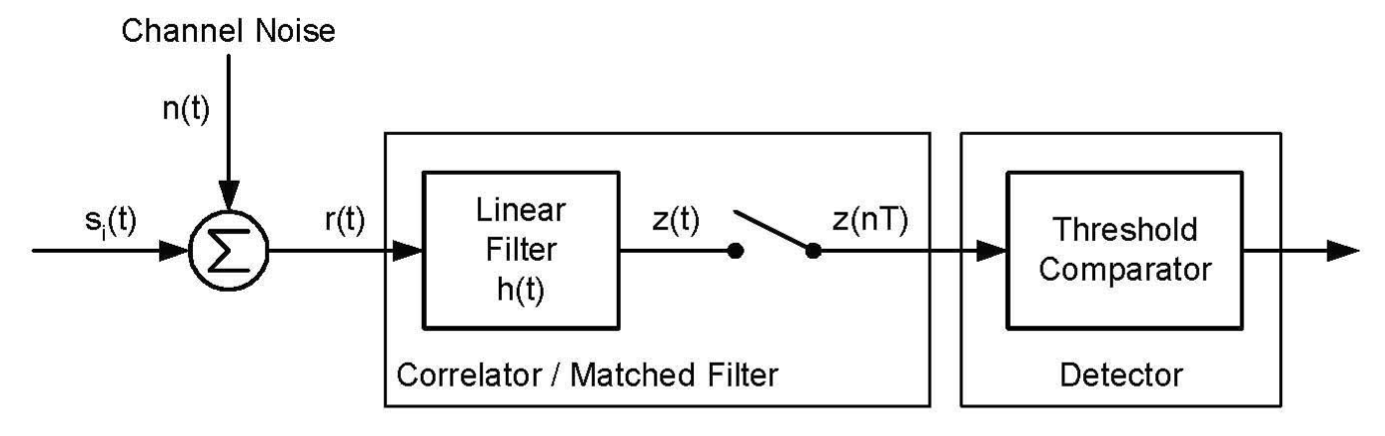
\includegraphics[height=3cm]{bilder/09_digital_signal_detection.png}
\end{center}

$$s_i(t) = \begin{cases}
          	s_1(t) & 0 \leq t \leq T \qquad \text{für Logisch } 1 \\
          	s_2(t) & 0 \leq t \leq T \qquad \text{für Logisch } 0          	
          \end{cases} 
				\qquad \overset{Rauschen}{\Longrightarrow} \qquad 
			r(t) = s_i(t) + n(t) 
				\qquad \overset{Filter}{\Longrightarrow} \qquad 
			z(t) = r(t) \ast h(t)$$ \\

\begin{enumerate}
  \item Am \textbf{Empfänger} $r(t)$ liegt das \textbf{Signal} $s(t)$ zusätzlich mit einem Additiven 
  		Weissen Gauss'schen (AWGN) \textbf{Rauschen} $n(t)$ vor.
  \item Mit dem \textbf{linearen Filter} wird das Signal-Rausch-Verhältnis (\textbf{SNR})
		\textbf{optimiert} (so \textbf{gross} wie möglich gemacht). Das Signal nach dem Filter sollte
		möglichst \textbf{wenig Rauschen} aber \textbf{viel Signalanteil} enthalten. \\
		Hierbei können zwei Strategien angewendet werden, das Matched Filter 
		\verweiskurz{09_matched_filter} oder der Korrelator
		\verweiskurz{09_korrelator}.
  \item Anschliessend wird das Signal \textbf{zeitdiskretisiert}, also immer nach einer konstanten Zeit
  		(Samplingzeit $t = T$) abgetastet. Dadurch resultiert: $z(T) = a_i(T) + n_0(T)$, wobei $a_i(T)$
  		dem Signalanteil und $n_o(T)$ dem Rauschanteil entspricht. \\
  		Dies entspricht zwei Normalverteilungen, welche um die Mittelwerte ($a_1, a_2$) angeordnet sind.
  \item Schlussendlich wird mit dem Schwellwertdetektor entschieden, welches Signal
  		höchstwahrscheinlich gesendet wurde. Man unterscheidet die zwei verschiedenen Arten von
  		Detektoren: \\ \textbf{Hard-Decision:} Das Resultat des Detektors ist eine endgültige
  		Entscheidung (0 oder 1). Die Entscheidung wird mit Hilfe des Schwellwerts $\lambda_0$ gefällt.\\ 
  		\textbf{Soft-Decision:} Für 0 und 1 werden Wahrscheinlichkeiten bestimmt und verarbeitet.
\end{enumerate}

\subsection{Optimaler Detektor}
\skriptsubsubsection{Hypothesen und Fehlerwahrscheinlichkeit}{227-9.2,3.A}
	Für die Entscheidung existieren zwei \textbf{Hypothesen} ($H_1 \Rightarrow s_1$ wurde gesendet, 
	$H_2 \Rightarrow s_2$ wurde gesendet): \\ 
	Falls das gesamplete Signal ($z(T) > \lambda_0$) ist, wird $H_1$, 
	für ($z(T) < \lambda_0$) wird $H_2$ gewählt. \\

\begin{minipage}[c]{10cm}
	\begin{center}
	 	\begin{tabular}{|l|c|c|}
			\hline
				gesendet $\backslash$ detektiert & Log. $1 = H_1$ & Log. $0 = H_2$ \\
			\hline
				Log. $1$ = $s_1$, mit $P(s_1)$ & $\textcolor{green}{P(H_1 | s_1)}$ 
												&  $\textcolor{red}{P(H_2 | s_1)}$\\
			\hline
				Log. $0$ = $s_2$, mit $P(s_2)$ & $\textcolor{red}{P(H_1 | s_2)}$ 
												& $\textcolor{green}{P(H_2 | s_2)}$ \\
			\hline
		\end{tabular}  
  	\end{center}
\end{minipage}
\begin{minipage}[c]{8cm}
	Die \textbf{Fehler-WSK} $P_e$ ist somit wie folgt definiert:
	$$ P_e = \textcolor{red}{P(H_2 | s_1)} P(s_1) + \textcolor{red}{P(H_1 | s_2)}
	P(s_2)$$
\end{minipage} 

\skriptsubsubsection{Maximum Likelihood Detektor}{227-9.3.B}
Bei einem Maximum Likelihood Detektor ist der Schwellwert $\lambda_0$ genau so gewählt, dass die
\textbf{Fehler-WSK }$P_e$ \textbf{minimal} wird. \\
Konkret kann dies berechnet werden, indem man das \textbf{Minimum} von $P_e$ bestimmt, also: $\qquad
\dfrac{d P_e}{d \lambda_0} = 0 \qquad$ setzt. \\ \\

\begin{minipage}[c]{9.5cm}
 	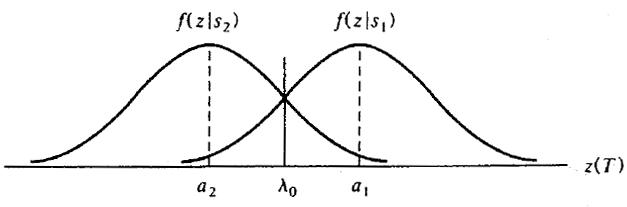
\includegraphics[width=8.5cm]{../NaT2/bilder/09_AWGN-PDF.png} \newline
 	$a_1 = $ Amplitude $\cdot T$ \newline
 	$a_2 = $ Amplidude $\cdot -T$
\end{minipage}
\begin{minipage}[c]{7cm}
	 $$ \lambda_0 = \dfrac{1}{2} (a_1 + a_2) + \dfrac{\sigma_{n_0}^2}{a_1 - a_2}
 \ln\dfrac{P(s_2)}{P(s_1)} $$ 
 	$$ \lambda_0 = \dfrac{a_1 + a_2}{2} \qquad (\text{gilt für: } P(s_2) = P(s_1) = \dfrac{1}{2})
 	$$
\end{minipage} 

Somit beträgt die Fehler-WSK: $ \qquad P_e = \textcolor{red}{P(H_2 | s_1)} P(s_1) + \textcolor{red}{P(H_1 | s_2)} = 
 P(s_1) \int\limits_{-\infty}^{\lambda_0} f(z|s_1) dz + P(s_2) \int\limits_{\lambda_0}^{\infty}
 f(z|s_2) dz$ \\
Mit ($P(s_2) = P(s_1) = \dfrac{1}{2}$) und ($\lambda_0 = \dfrac{a_1 + a_2}{2}$) gilt für ein
\textbf{NRZ-Signal}: $ \qquad P_e = Q \left(\dfrac{a_1 - a_2}{2 \sigma_{n_0}}\right) $



\subsection{Lineares Filter}
\skriptsubsubsection{Matched Filter}{229-9.4.A} \label{09_matched_filter}
	\textbf{Ziel: } Maximierung von $(a_1 - a_2)$ bei gleichzeitiger Minimierung
	von $n_0$. Mit $E_{s(t)}$ als Energie des Eingangssignals $s(t)$.
	%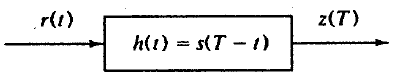
\includegraphics[width=4.5cm]{../NaT2/bilder/09_matched_filter.png}
 
	$$\text{SNR wird maximal bei} H \left( \omega \right) = S^* \left( \omega
	\right) \e^{-\jmath \omega T} \quad \IFT \quad h \left( t \right) = 
	\begin{cases} s(T-t) & 0 \leq t \leq T \\
	0 & sonst\end{cases} \qquad \text{wobei } \left(\dfrac{S}{N}\right)_{0_{max}} =
	\dfrac{2E_{s(t)}}{\eta}$$
 	

\skriptsubsubsection{Korrelator}{230-9.4.B} \label{09_korrelator}
Für den Sample Zeitpunkt ($t=T$) sind die Eigenschaften eines \textbf{Matched-Filter} und diejenigen eines
\textbf{Korrelators} \textbf{identisch}. Somit können beide für den selben Zweck eingesetzt werden.

$$ z(t) = r(t) \ast h(t) = \int_0^t r(\tau) h(t-\tau) d\tau \overbrace{=}^{h(t) =
h_{MatchedFilter}(t)} \int_0^t r(\tau) s[T - (t - \tau)] d\tau \overbrace{=}^{t = T} \int_0^T
r(\tau)s(\tau)$$

	\begin{center}
		\begin{minipage}[c]{4.5cm}
			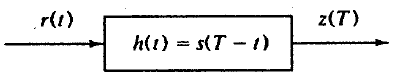
\includegraphics[width=4.5cm]{../NaT2/bilder/09_matched_filter.png}
		\end{minipage}
		\begin{minipage}[c]{2cm}		
			$$\Longleftrightarrow $$
		\end{minipage}
		\begin{minipage}[c]{4.5cm}
			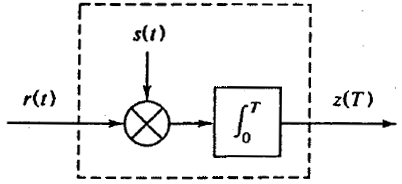
\includegraphics[width=4.5cm]{../NaT2/bilder/09_correlator.png}
		\end{minipage}
	\end{center}

\skriptsubsubsection{Unmatched RC-Filter}{238-Prob.9.9}
Hierbei wird an Stelle eines Matched Filters ein RC-Tiefpassfilter verwendet. \\
$$H(\omega) = \dfrac{1}{1 + j \omega R C}$$
% \qquad \dfrac{T}{RC} = 1.257 \qquad
%\left(\dfrac{S}{N}\right)_0_{max} = (0.815)\dfrac{2 A^2 T}{\eta}$$

\skriptsubsection{Fehlerwahrscheinlichkeit verschiedener binären
Übertragungen}{231-9.5}\label{09_binary_signals_error}
\small{$E_b$ bezeichnet die mittlere Signalenergie pro Bit.}\\
\renewcommand{\arraystretch}{2.5}
	\begin{tabular}{ p{6cm} p{2.5cm} p{9cm} }		
		\multicolumn{3}{l}{\textbf{Unipolar Baseband Signaling}} \\
		$ P_e = Q\left(\sqrt{\dfrac{A^2 T}{2 \eta}}\right) = Q\left(\sqrt{\dfrac{E_b}{\eta}}\right) $
		& $ E_b = \dfrac{A^2 T}{2} $
		& $ s_i(t) = \begin{cases}
		     s_1(t) = A & 0 \leq t \leq T \\       
		     s_2(t) = 0 & 0 \leq t \leq T
		   \end{cases}$ \\  

		\multicolumn{3}{l}{\textbf{Bipolar Baseband Signaling}} \\
		$ P_e = Q\left(\sqrt{\dfrac{2 A^2 T}{\eta}}\right) = Q\left(\sqrt{\dfrac{2 E_b}{\eta}}\right) $
		& $ E_b = A^2 T $
		& $ s_i(t) = \begin{cases}
 		     s_1(t) = +A & 0 \leq t \leq T \\       
 		     s_2(t) = -A & 0 \leq t \leq T
 		   \end{cases} $ \\

		\multicolumn{3}{l}{\textbf{Amplitude-Shift Keying}} \\
		$ P_e = Q\left(\sqrt{\dfrac{A^2 T}{4 \eta}}\right) = Q\left(\sqrt{\dfrac{E_b}{\eta}}\right) $
		& $ E_b = \dfrac{A^2 T}{4} $
		& $ s_i(t) = \begin{cases}
 		     s_1(t) = A \cos{\omega_c t} & 0 \leq t \leq T \\       
 		     s_2(t) = 0 & 0 \leq t \leq T
 		   \end{cases} $ \\

		\multicolumn{3}{l}{\textbf{Phase-Shift Keying}} \\
		$ P_e = Q\left(\sqrt{\dfrac{A^2 T}{\eta}}\right) = Q\left(\sqrt{\dfrac{2 E_b}{\eta}}\right)  $
		& $ E_b = \dfrac{A^2 T}{2} $
		& $ s_i(t) = \begin{cases}
 		     s_1(t) = A \cos{\omega_c t} & 0 \leq t \leq T \\       
 		     s_2(t) = A \cos{(\omega_c t + \pi)} = - A \cos{\omega_c t} & 0 \leq t \leq T
 		   \end{cases} $ \\

		\multicolumn{3}{l}{\textbf{Frequency-Shift Keying}} \\
		$ P_e = Q\left(\sqrt{\dfrac{A^2 T}{2 \eta}}\right) = Q\left(\sqrt{\dfrac{E_b}{\eta}}\right) $
		& $ E_b = \dfrac{A^2 T}{2} $
		& $ s_i(t) = \begin{cases}
 		     s_1(t) = A \cos{\omega_1 t} & 0 \leq t \leq T \\       
 		     s_2(t) = A \cos{\omega_2 t} & 0 \leq t \leq T
 		   \end{cases}$ \\

 	\end{tabular}
	\renewcommand{\arraystretch}{1}
